\begin{frame}{RTDroid - Message Channel}
	\only<3>{\centering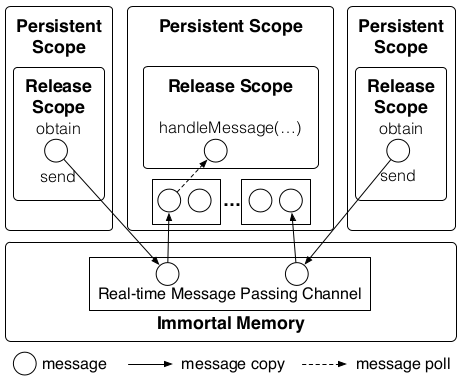
\includegraphics[scale=0.40]{messageChannel}}
	\only<1>{\begin{itemize}
		\item Limitato numero di messaggi in attesa (destinatario)
		\item Trasferibili solo array di tipi primitivi o buffer di byte a dimensione fissa
		\begin{itemize}
			\item In questo modo si mantiene controllata l'occupazione di memoria
		\end{itemize}
		\item I messaggi vengono preallocati sulla base della dimensione del canale 
		\item Se non ci sono messaggi disponibili un thread ad alta priorità può ''rubare'' un messaggio
	\end{itemize}}
	\only<2>{\begin{itemize}
		\item Il ricevente copia il payload nella sua memoria solo quando accetta il messaggio
		\begin{itemize}
			\item Messaggi accettati uno alla volta
			\item La memoria occupata nel ricevente è tenuta sotto controllo e pulita dopo ogni gestione (release memory)
			\item Una volta ricevuto, il messaggio torna disponibile
		\end{itemize}
		\item Il ricevente non può essere intasato da messaggi in entrata
		\item I messaggi accodati non sono ancora stati ricevuti, quindi è safe prelevarne uno a bassa priorità
		\begin{itemize}
			\item Il derubato verrà notificato con una eccezione
			\item Il framework assicura che nessun componente abbia un riferimento diretto al messaggio
			\item Chi ha priorità alta non viene bloccato
		\end{itemize}
	\end{itemize}}
\end{frame}